% Náhled k~sekci o~výrokové logice: pravdivostní tabulka základních spojek.
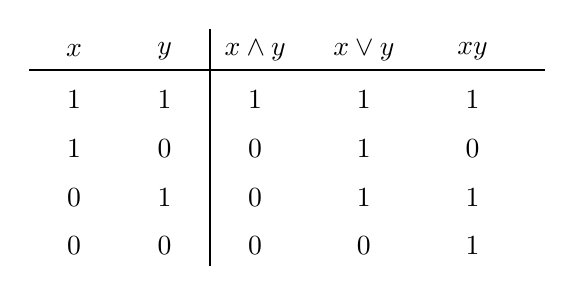
\begin{tikzpicture}[x=1.15cm, y=0.62cm]

    \tikzset{
        hdr/.style={font=\bfseries},
        one/.style={fill=darkgreen!18},
        zero/.style={fill=darkred!12}
    }

    % záhlaví
    \node[hdr] at (0,0) {$x$};
    \node[hdr] at (1,0) {$y$};
    \node[hdr] at (2,0) {$x\land y$};
    \node[hdr] at (3.2,0) {$x\lor y$};
    \node[hdr] at (4.4,0) {$x\implies y$};

    \draw[thick] (-0.5,-0.4) -- (5.2,-0.4);
    \draw[thick] (1.5,0.45) -- (1.5,-4.4);

    % řádky: x, y, and, or, imp
    \foreach \r/\x/\y/\a/\o/\i in {
        1/1/1/1/1/1,
        2/1/0/0/1/0,
        3/0/1/0/1/1,
        4/0/0/0/0/1}
    {
        \node at (0,-\r) {$\x$};
        \node at (1,-\r) {$\y$};
        \node at (2,-\r) {$\a$};
        \node at (3.2,-\r) {$\o$};
        \node at (4.4,-\r) {$\i$};
    }

\end{tikzpicture}
